\subsection{Determination of the Proton Resonance Frequency Using the Lock-in Method}
As already discussed in the "Theoretical Background" chapter, to determine the resonance frequency of a proton in hydrogen using the lock-in method, the zero passages of the sine-overlapped sawtooth voltage and the derived absorption curve had to be measured. The time difference of these had to be determined for different frequencies in order to be able to do a linear fit, with which it was possible to determine the resonance frequency (that's the frequency at $\Delta t=0s$). The frequencies for which we did a measurement can be found in the appendix: as one can see, we decided to neglect the second and third measurement as the chosen frequencies were above the resonance frequency determined in part 2 of the experiment. \\
We determined the zero passage of the derived absorption curve by looking at the two values around the passage. We took the time attached to the closer one and an uncertainty of $s_{t_{abs}}=0,002 s$ as there is a measurement every 0,002 seconds and there might be a deviation for the voltage measured, making it hard to determine the point neighboring the zero passage which is actually closer to 0: this is why we decided to take this uncertainty, the time between two measurements. As for the sine-overlapped sawtooth voltage it was quite hard to determine a zero passage, we decided to determine the period of the signal and add half of it onto the lower end (the start)  of the signal. \\
The period was determined as can be seen below:\\
\[T=t_{top}-t_{bottom}\] where $t_{top}$ stands for the time attached to the maximum voltage and $t_{bottom}$ for the time attached to the minimum voltage reached by the sine-modulated sawtooth signal. Again, we decided to use an uncertainty of $s_{t_ {top}}=s_{t_{bottom}}=0,002 s$ because we don't know about what is happening between the minimum and the maximum of the signal and therefore can't decide, where the actual starting and ending points are. Therefore, the resulting uncertainty can be calculated the following way:\\
\[s_{T}=\sqrt{s_{t_{top}}^{2}+s_{t_{bottom}}^{2}}\]
The period was determined 6 times: we would get $T=5,251 s$ in every measurement. The resulting uncertainty reduces to \[s_{\bar{T}}=\frac{\sqrt{s_{t_{top}}^{2}+s_{t_{bottom}}^{2}}}{\sqrt{6}},\] whereas the period is \[\bar{T}=\frac{1}{6}\sum\limits_{i=1}^{6}T_{i}=5,251 s.\]
As the uncertainty on $t_{bottom}$, $s_{t_{bottom}}=0,2 s$ is not independent of the uncertainty on $\bar{T}$ and that uncertainty is smaller, we decided to neglect $s_{\bar{T}}$, when determining the uncertainty on \[t_{0_{sawtooth}}=t_{bottom}+\bar{T},\] making the resulting uncertainty look like the following:\[s_{t_{0_{sawtooth}}}\approx s_{t_{bottom}}\]
\clearpage
A measurement can be seen below:\\
\begin{figure}[htbp]
\begin{center}
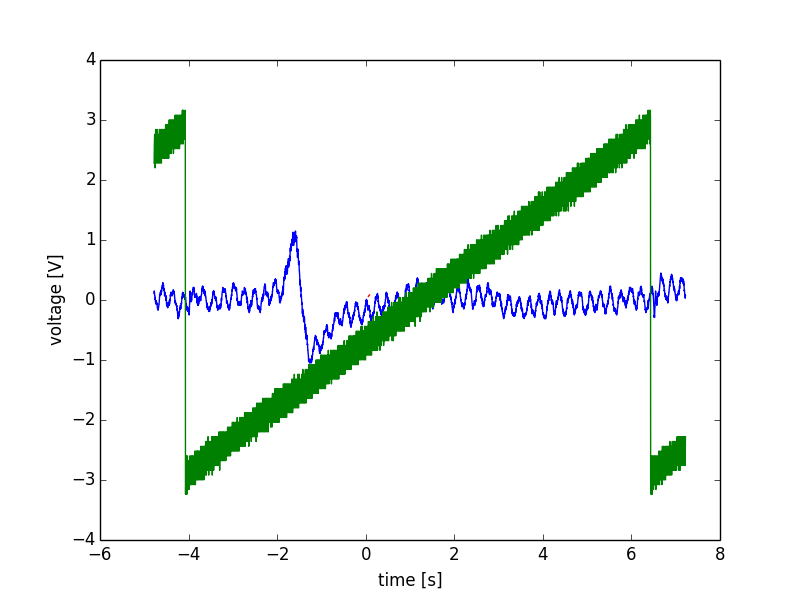
\includegraphics{saege}
\caption{Sine-overlapped sawtooth signal (green) and resulting derived absorption curve (blue)}
\end{center}
\end{figure}
\clearpage
This fits the theoretical expectation, which can be found in the "Theoretical Background" chapter, well.\\
To determine $\Delta t$, we have to calculate the difference between the zero passages of the sine-overlapped sawtooth and the derived absorption signal: \[\Delta t=t_{0_{sawtooth}}-t_{0_{abs}}\] with\\
 \[s_{\delta t}=\sqrt{s_{t_{0_{sawtooth}}}^{2}+s_{t_{0_{abs}}}^{2}}\]
 With the formula and the method explained above we got the following results:\\
 \begin{table}[htbp]
 \begin{center}
 \begin{tabular}{|r|r|r|r|}
 \hline
 \multicolumn{1}{|l|}{f in MHz} & \multicolumn{1}{l|}{$s_{f}$ in MHz} & \multicolumn{1}{l|}{$\Delta t$ in s} & \multicolumn{1}{l|}{$s_{\Delta t}$ in s} \\ \hline
 17,624 & 0,01 & 0,271 & 0,00283 \\ \hline
 17,618 & 0,01 & 0,285 & 0,00283 \\ \hline
 17,6042 & 0,01 & 2,219 & 0,00283 \\ \hline
 17,5998 & 0,01 & 4,195 & 0,00283 \\ \hline
 17,5797 & 0,01 & 4,315 & 0,00283 \\ \hline
 17,6019 & 0,01 & 3,475 & 0,00283 \\ \hline
 17,5892 & 0,01 & 4,017 & 0,00283 \\ \hline
 \end{tabular}
 \end{center}
 \end{table}
 
 We used the displayed values to do our linear fit. The uncertainty we attach to the frequency has already been discussed. Using this values, we did the linear fit mentioned. It can be seen below:\\
 \begin{figure}[htbp]
 \begin{center}
 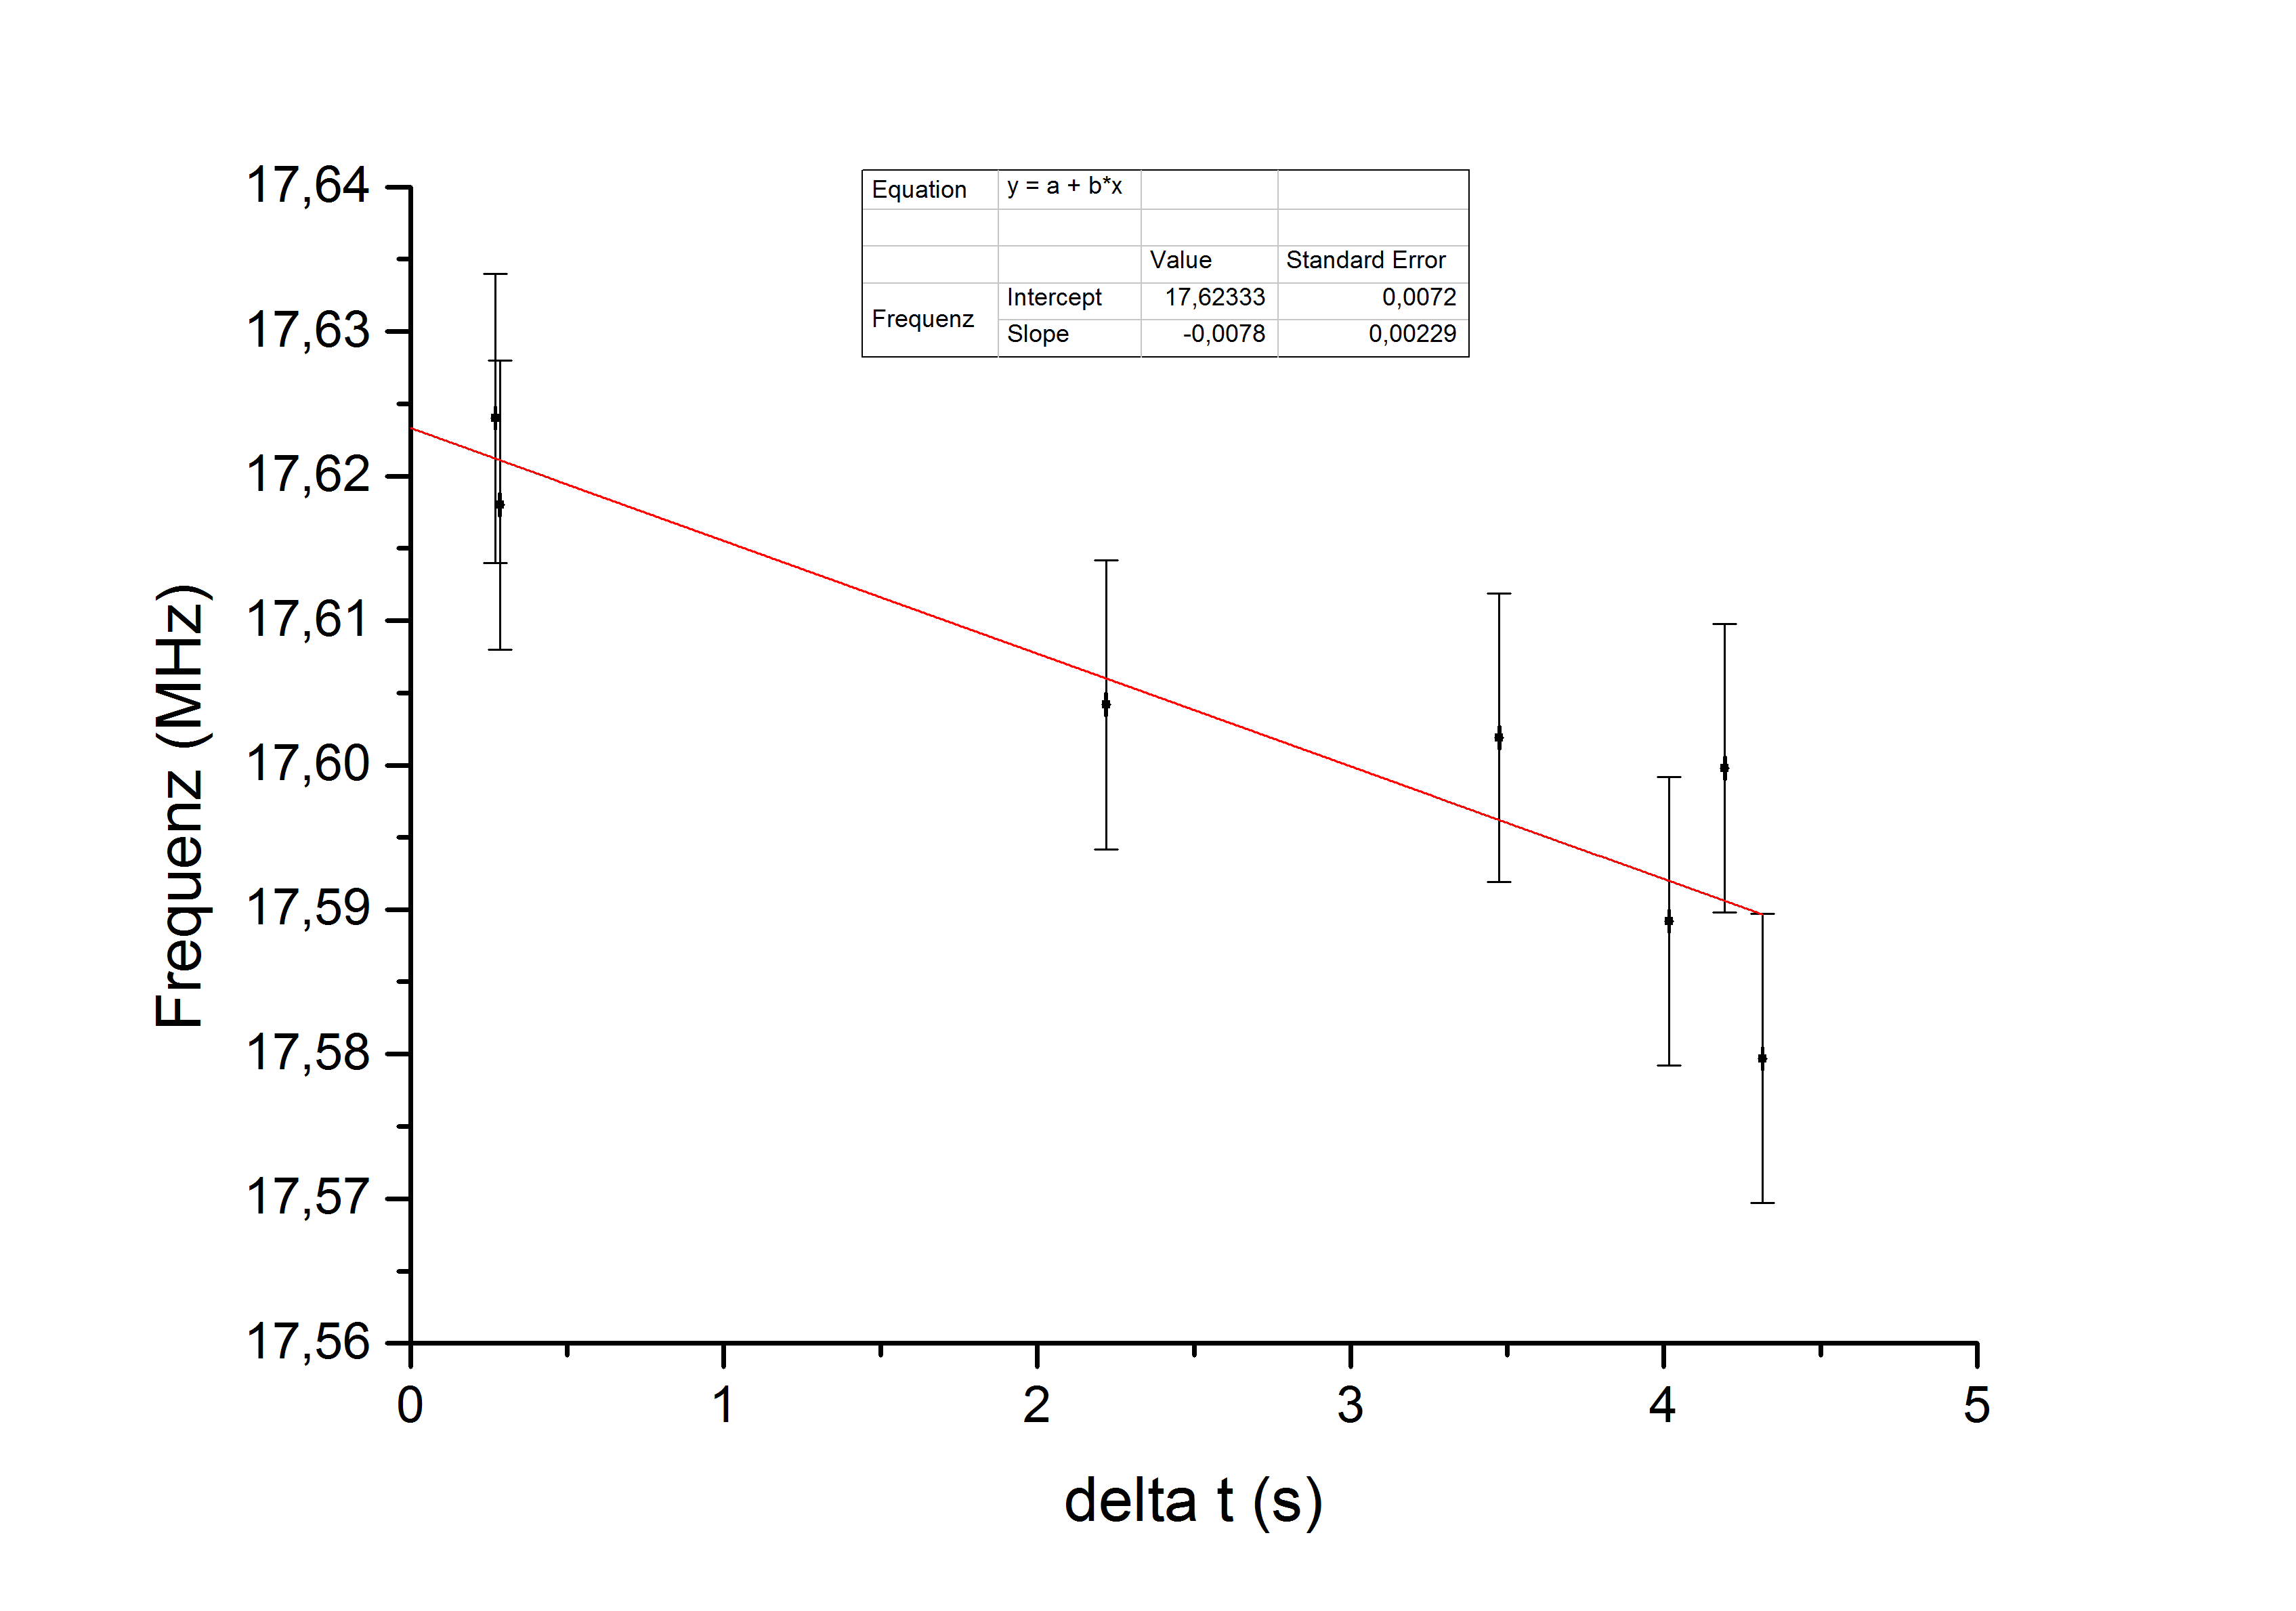
\includegraphics[scale=0.5] {Bilder/linfit}
 \caption{Linear fit used for the determination of the resonance frequency}
 \end{center}
 \end{figure}
 \clearpage
 The scattering of the measured values is quite large due to the fact that the frequency couldn't be determined very accurately. \\
The resonance frequency we determined using this method is $\nu=(17,623\pm0,007) MHz$. Using $B=(419\pm0,8)mT$, for the gyromagnetic ratio we get:\\
\[\nu=\frac{\gamma\cdot B}{2\pi}\]
\[\Leftrightarrow \gamma=\frac{\nu\cdot2\pi}{B}\]
\[\Rightarrow s_{\gamma}=\sqrt{(\frac{\partial \gamma}{\partial B})^{2}\cdot s_{B}^{2}+(\frac{\partial\gamma}{\partial\nu})^{2}\cdot s_{\nu}^{2}}=\sqrt{\frac{4\pi^{2}\cdot\nu^{2}}{B^{4}}\cdot s_{B}^{2}+\frac{4\pi^{2}}{B^{2}}\cdot s_{\nu}^{2}}\]
With this formula, using the lock-in method we get the following for the gyromagnetic ratio:\\
$\gamma=(2,643\pm0,005)\cdot 10^{8}\frac{1}{s\cdot T}$ \\
A discussion of this result can be found in the chapter "Conclusion".